\section{Mätinstrument}
\textbf{
  HAREC a.\ref{HAREC.a.8.2}\label{myHAREC.a.8.2}
}

\subsection{Att mäta är att veta}

Mätinstrument används för att, under kontrollerade former, testa och bekräfta
en funktion eller avsaknad av densamma, i en utrustning.
Det används också för att mäta olika komponenter för att verifiera dess
funktion och egenskaper.

Med mätinstrument vill man åstadkomma en så snarlik testmiljö som man kan
förvänta sig, att utrustningen som man testar, ska kunna hantera i
verkligheten.

De mätinstrument vi kommer att nämna nedan, används bl.a. i en sluttester i de
fabriker, som när, i vårt fall, radioutrustningen är hopmonterad och ska
testas, innan den levereras till kund.

Att tillverkarna använder mätinstrument enligt ovan, är sålunda en
förutsättning för att kunna veta att den utrustning man konstruerat uppfyller
de krav som man specificerat.

Dessa typer av instrument är också av intresse för sändaramatören, då han / hon
kan använda dessa för felsökning eller service.

\subsection{Presentation av mätvärden}

\begin{wrapfigure}[20]{R}{0.5\textwidth}
  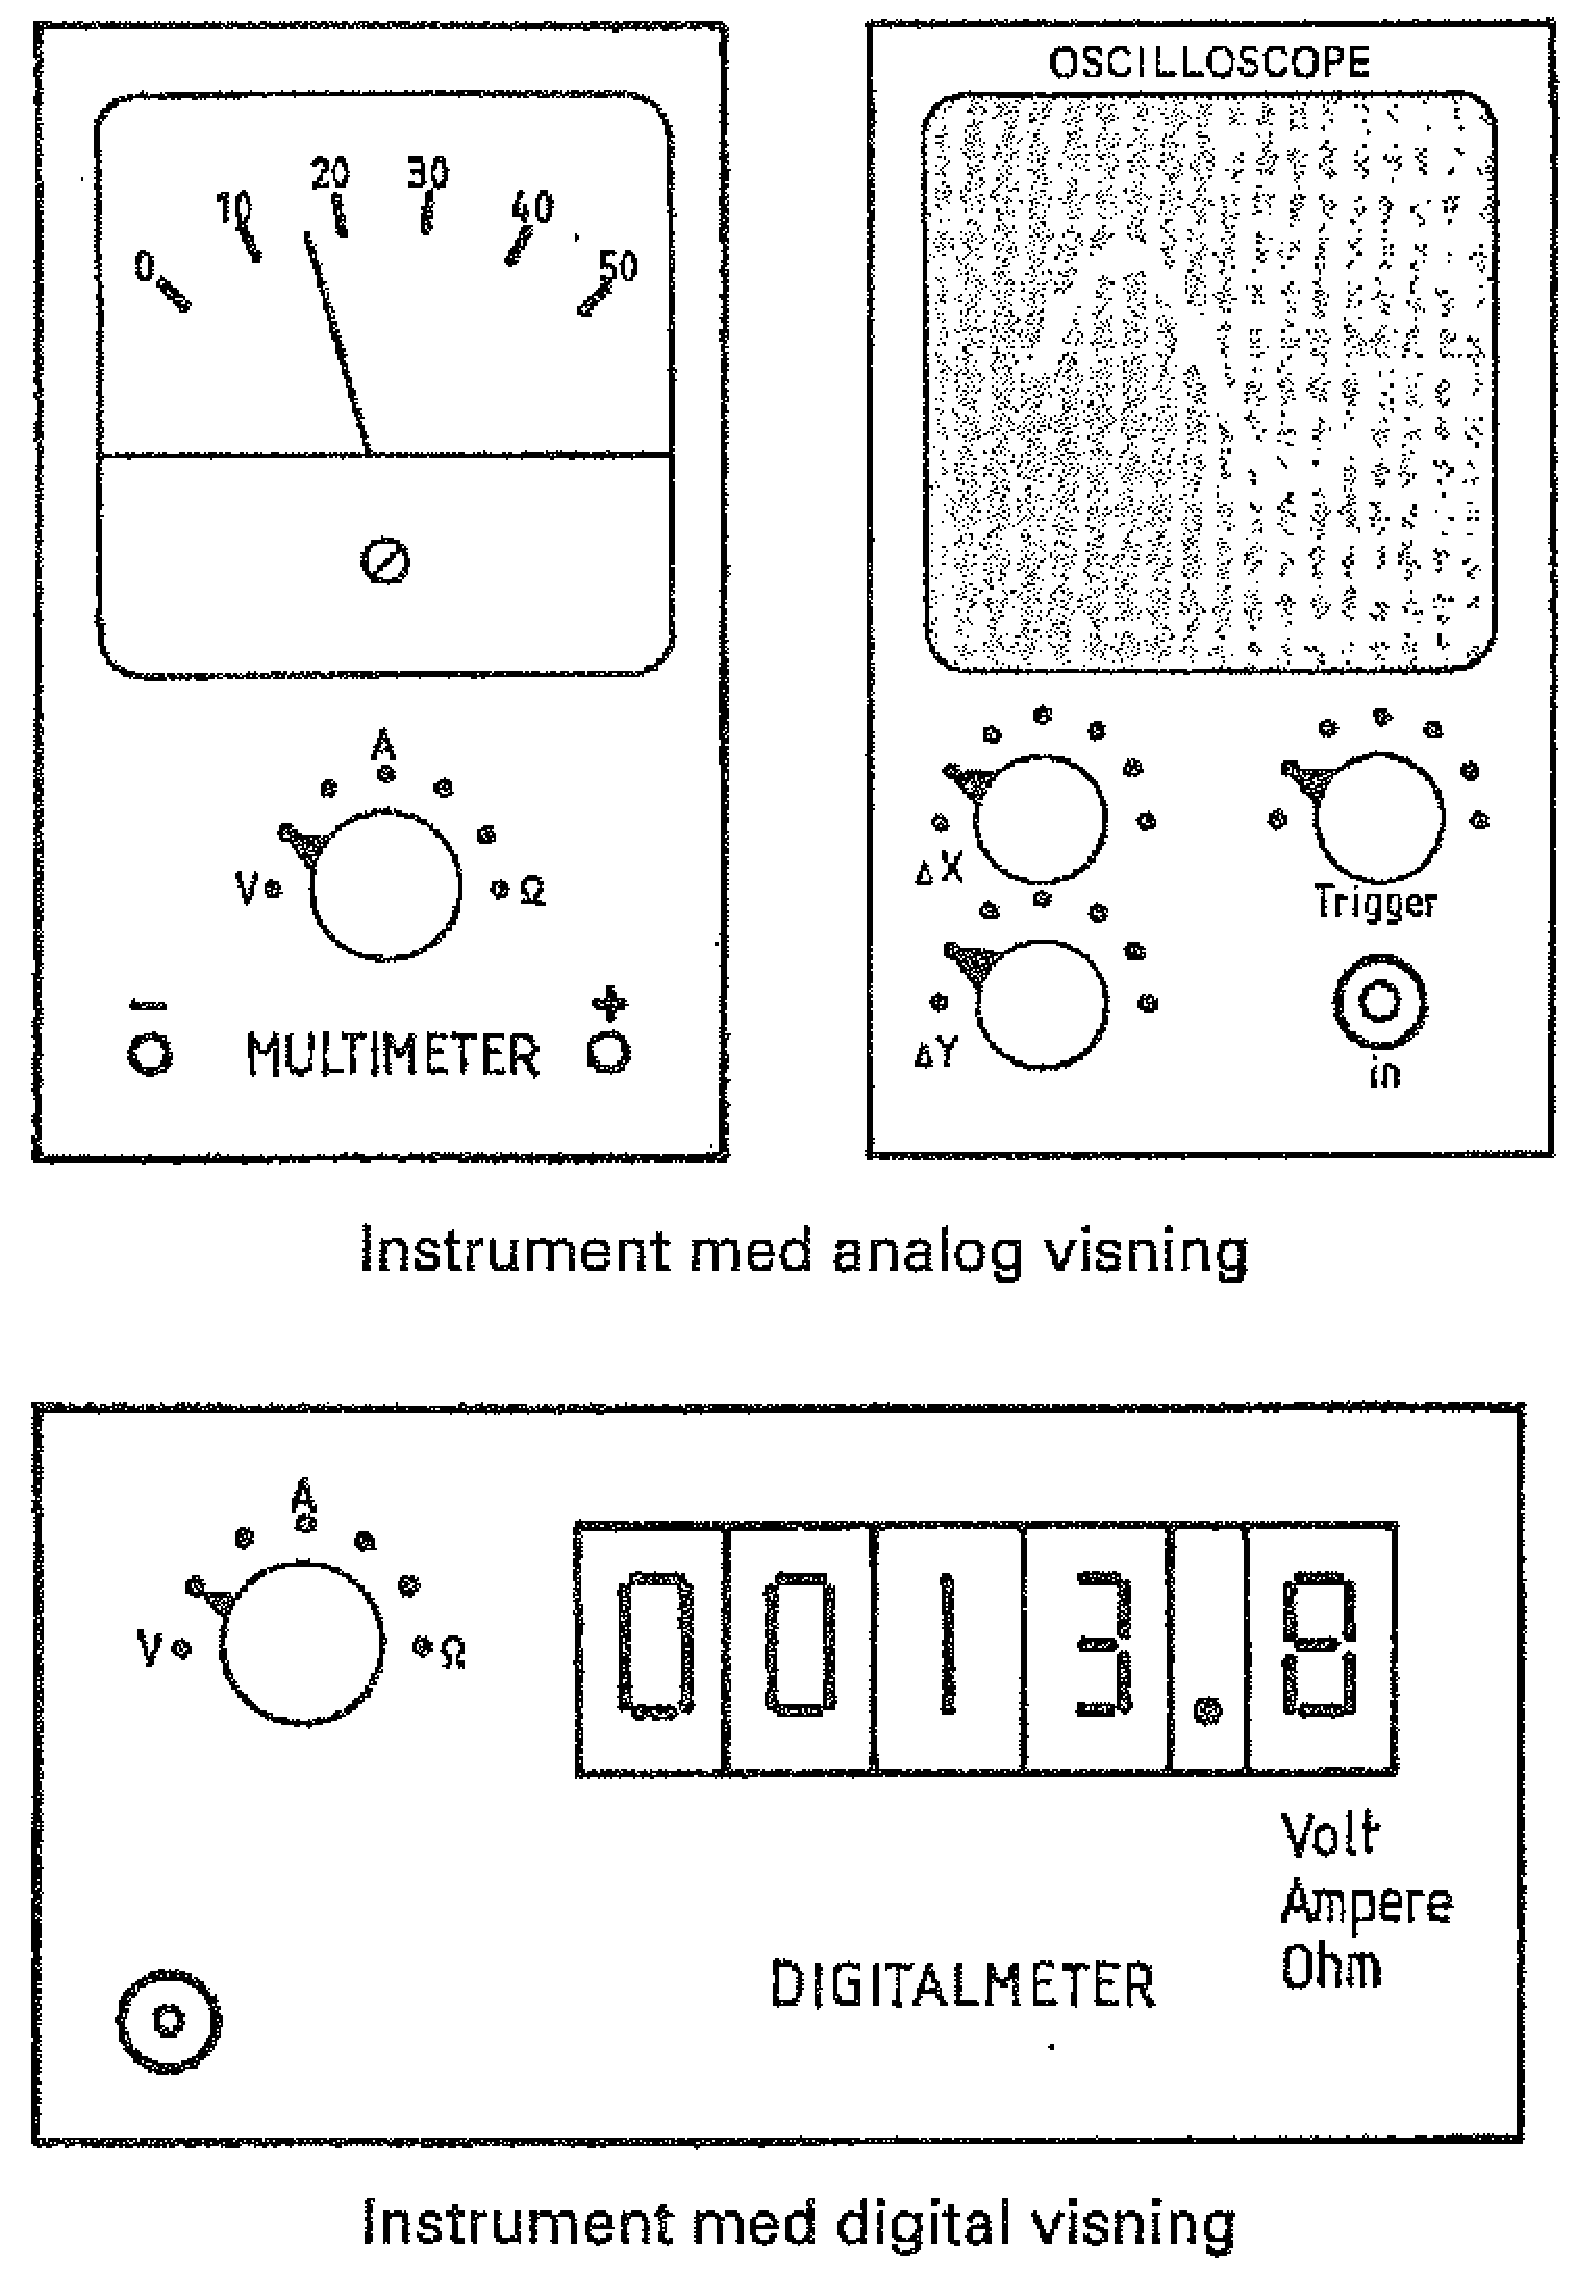
\includegraphics[width=0.5\textwidth]{images/cropped_pdfs/bild_2_8-02.pdf}
  \caption{Presentation av mätvärden}
  \label{fig:bildII8-2}
\end{wrapfigure}

Mätvärden kan presenteras på olika sätt som illustreras i bild
\ref{fig:bildII8-2}.
De vanligaste sätten är optiska och då med digital eller analog visning.
Mätresultat kan även överföras till dator för vidare bearbetning och visning.

\subsection{Multimeter}
\textbf{
HAREC a.\ref{HAREC.a.8.2.1.1}\label{myHAREC.a.8.2.1.1}
}
\index{multimeter}


Flera mätfunktioner kan utföras med samma basinstrument, som visas i
bild \ref{fig:bildII8-2}, denna egenskap kallas för en \emph{multimeter}.
Genom omkoppling mellan olika tillsatser väljer man mätfunktion och mätområde.
Instrumentskalan utformas så att olika slags mätvärden kan avläsas.
Kombinationer med elektroniska förstärkare och digital visning etc. är nu
vanligt.

\subsection{Vridspoleinstrument}
\index{vridspoleinstrument}

\begin{figure}
  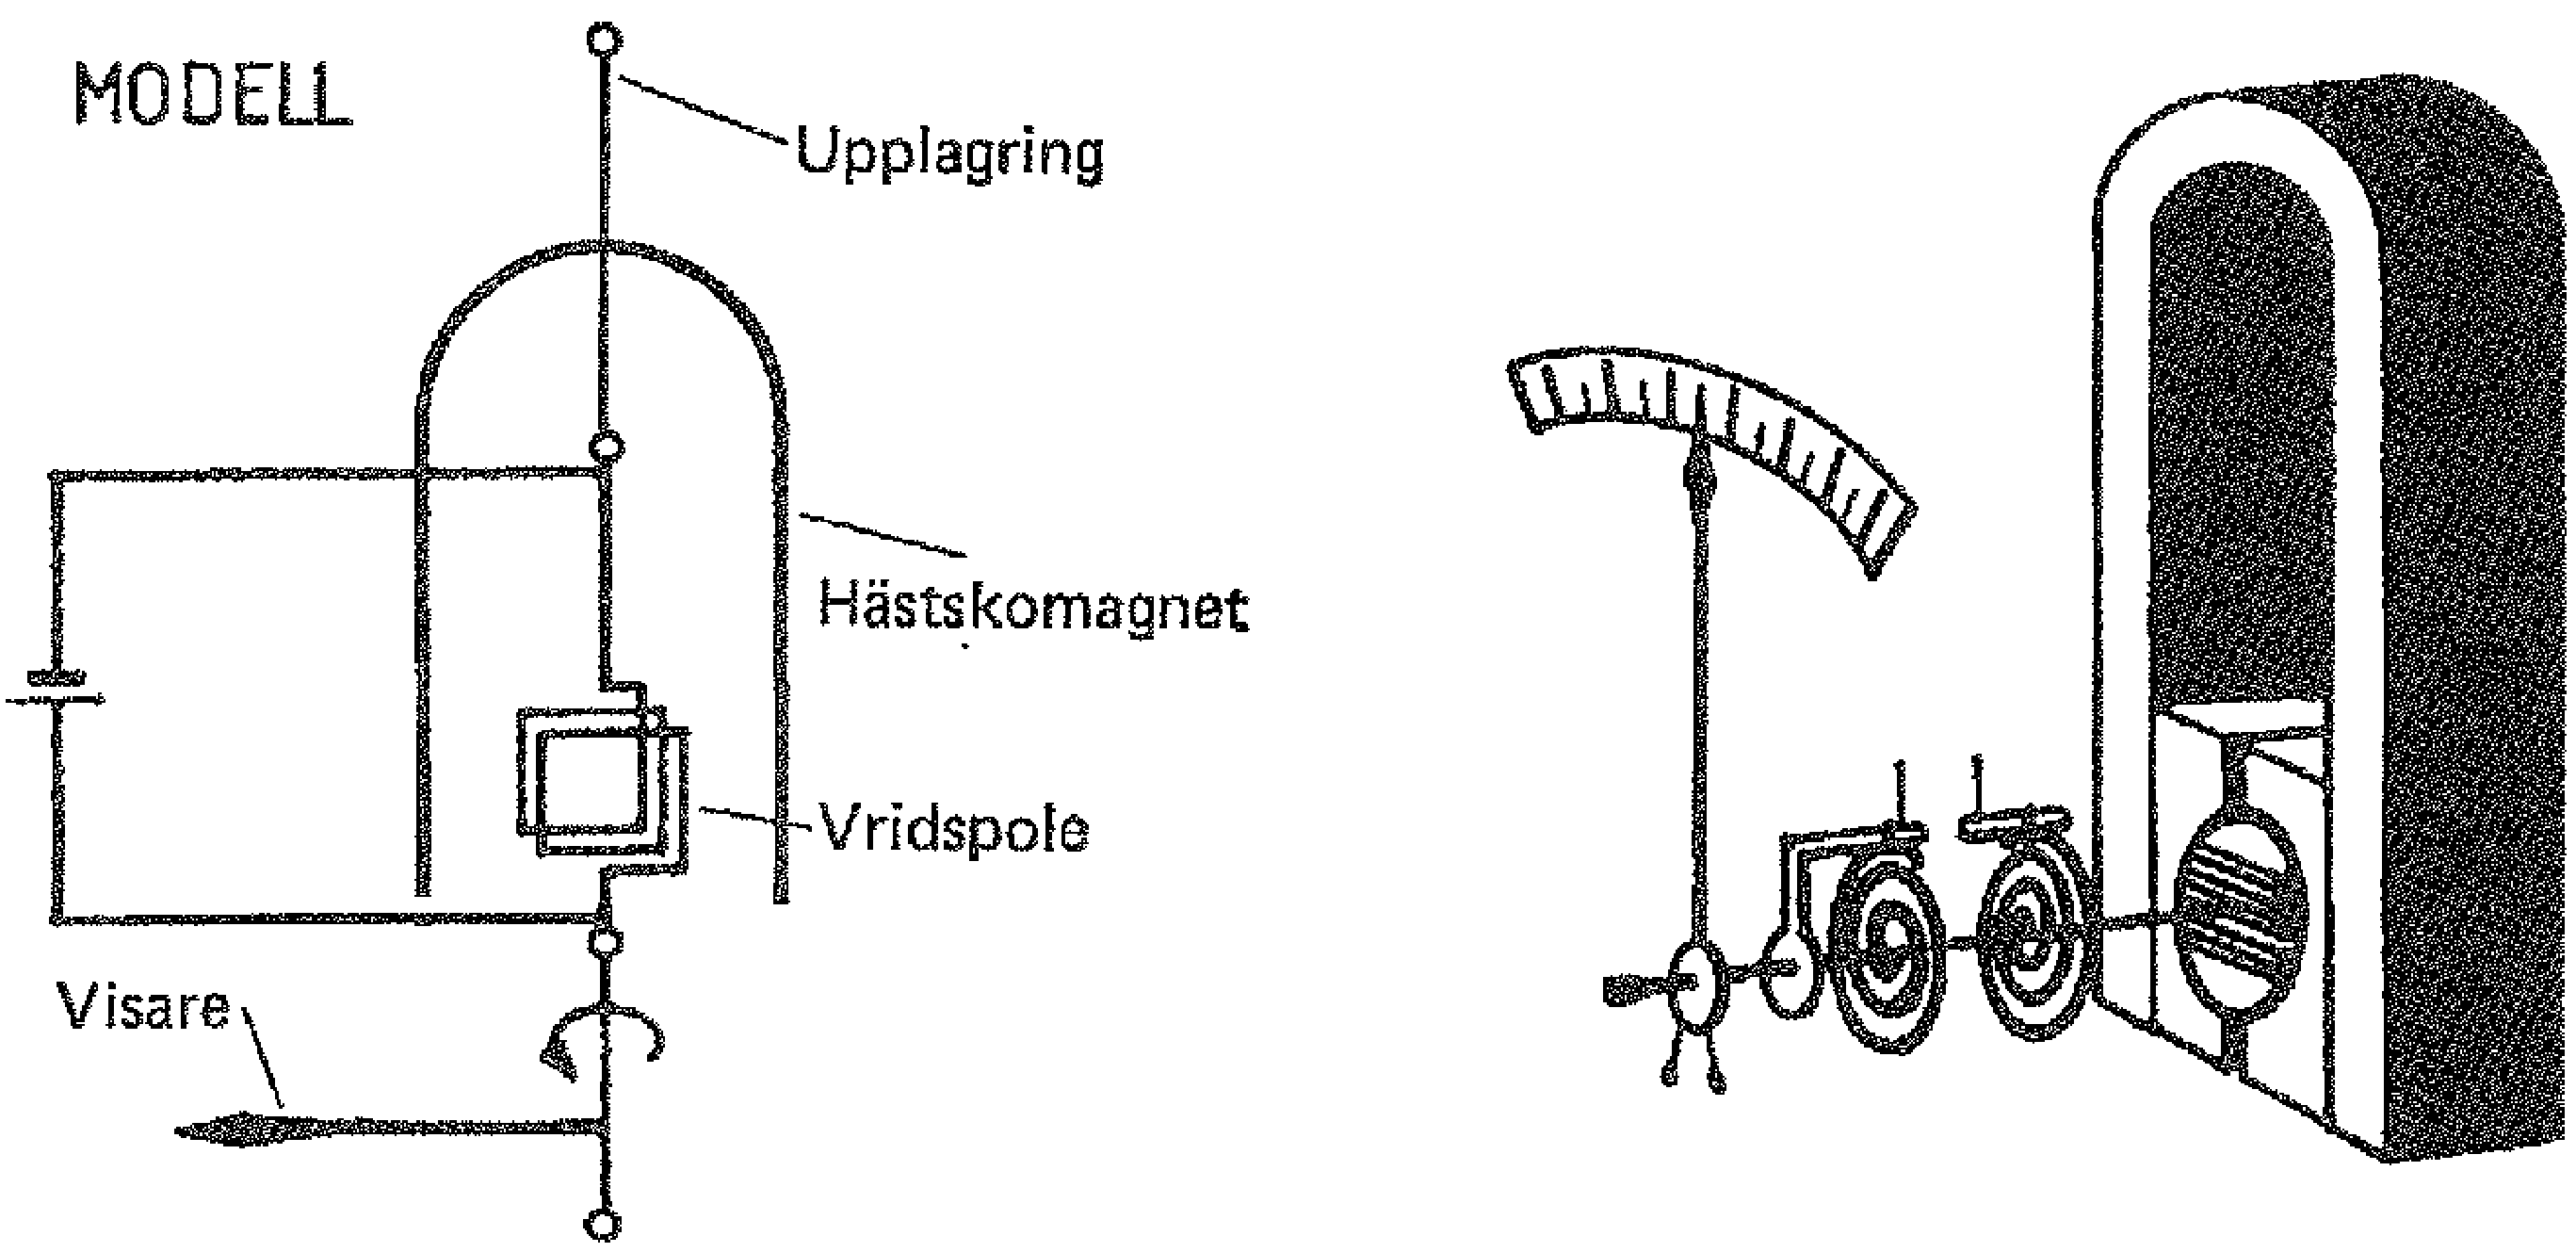
\includegraphics[width=\textwidth]{images/cropped_pdfs/bild_2_8-03.pdf}
  \caption{Vridspoleinstrument}
  \label{fig:bildII8-3}
\end{figure}

\emph{Vridspoleinstrument}, som illustreras i bild \ref{fig:bildII8-3}, kan
bara användas för likströmsmätning, eftersom visarutslaget beror av
strömriktningen.
Instrumentet har låg effektförbrukning och stor noggrannhet.
Visningen är vanligen linjär, men kan göras annorlunda.

\textbf{Funktion:}
En spole är upplagrad i fältet av en hästskomagnet.
När den ström, som ska mätas, passerar genom den vridbara spolen så alstras
ett magnetfält även i denna.
De två magnetfälten påverkar varandra så att spolen vrider sig.
Spolen förses med en visare och en returfjäder.
Ju större ström det flyter genom spolen desto större blir visarutslaget.

\begin{wrapfigure}{R}{0.5\textwidth}
  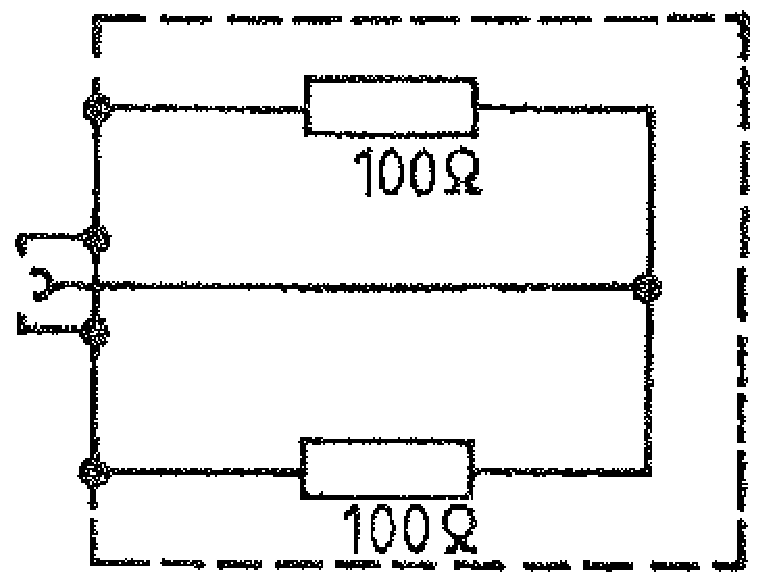
\includegraphics[width=0.5\textwidth]{images/cropped_pdfs/bild_2_8-05.pdf}
  \caption{Konstlast}
  \label{fig:bildII8-5}
\end{wrapfigure}

\subsection{Konstlast}
\index{konstlast}
\index{dummy load}

En \emph{konstlast} (eng. \emph{dummy load}) är en alternativ last som kan
hantera en viss mängd effekt, konstlast illustreras i bild \ref{fig:bildII8-5}.
En konstlast bör ingå i varje amatörradiostation.
Vid mätning och inställning av till exempel modulation och uteffekt, är det lämpligt
att belasta sändaren med dess nominella utgångsimpedans.
För att då undvika att energi strålas ut bör en väl skärmad konstlast användas.

I moderna amatörradiosändare med koaxialkabel utgång är utgångsimpedansen
50~\(\Omega\).
Konstlasten ska då vara en 50~\(\Omega\) resistor utan reaktiva egenskaper
för det intressanta frekvensområdet.
Den kan bestå av en eller flera sammankopplade resistorer, ofta parallellt för
att minska den induktiva komponenten.

Sändareffekten ska kunna tas upp utan att resistansen förändras nämnvärt.
Det är viktigt att resistorerna kyls effektivt med luft eller vätska i ett kärl
med tillräckligt utrymme, även när vätskan expanderar av värmen.
Vätskan får inte vara lättantändlig eller miljöfarlig.
Till exempel är oljor med PCB förbjudna!

\subsection{Fältstyrkemätare}
\index{fältstyrkemätare}

\begin{figure}
  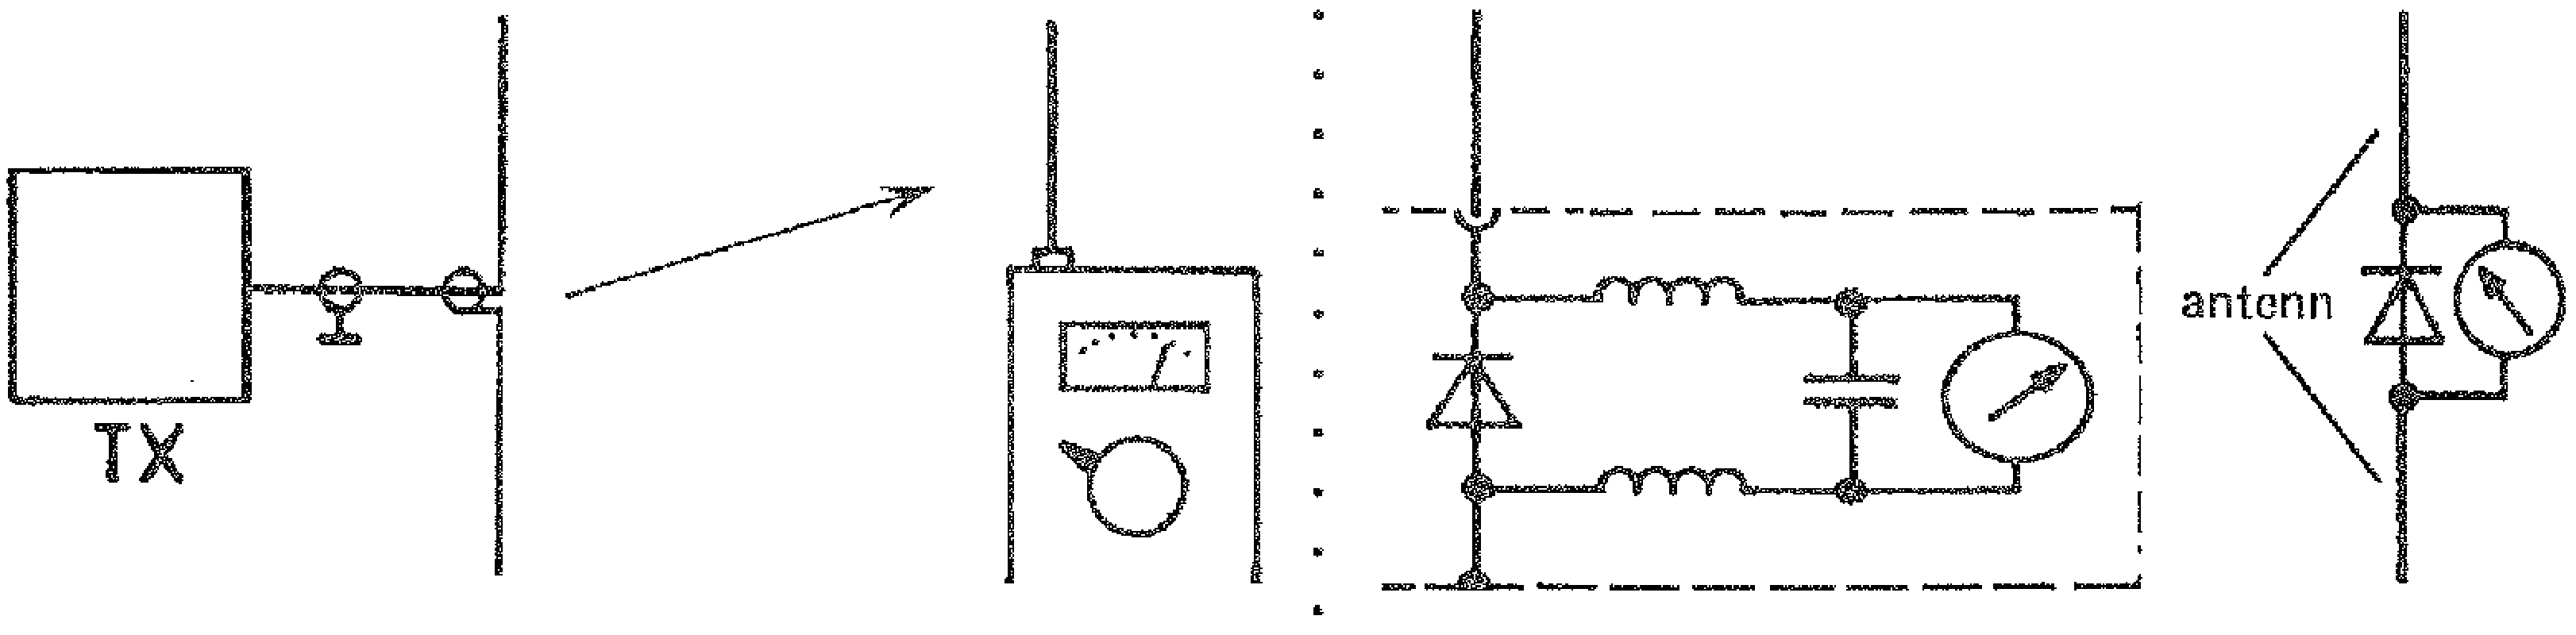
\includegraphics[width=\textwidth]{images/cropped_pdfs/bild_2_8-06.pdf}
  \caption{Fältstyrkemätare}
  \label{fig:bildII8-6}
\end{figure}

Styrkan av elektromagnetiska fält kan bestämmas med \emph{fältstyrkemätare}.

En fältstyrkemätare är en högfrekvensdetektor, vars utspänning visas med ett
instrument med skala.
Den selektiva kretsen kan bestå enbart av den avstämda antennen, men även av
ytterligare selektiva kretsar.
Instrumentet visar endast relativa värden och används till exempel för att bestämma
strålningsegenskaperna i sändarantenner och för antennjustering.
Mätresultatet påverkas även av utstrålning från andra sändare inom mätarens
bandbredd.
Bild \ref{fig:bildII8-6} visar en sändare och en fältstyrkemätare.
Dessutom två enkla fältstyrkemätare.

\subsection{Kalibreringsoscillator}
\index{kalibreringsoscillator}

\begin{wrapfigure}[12]{R}{0.5\textwidth}
  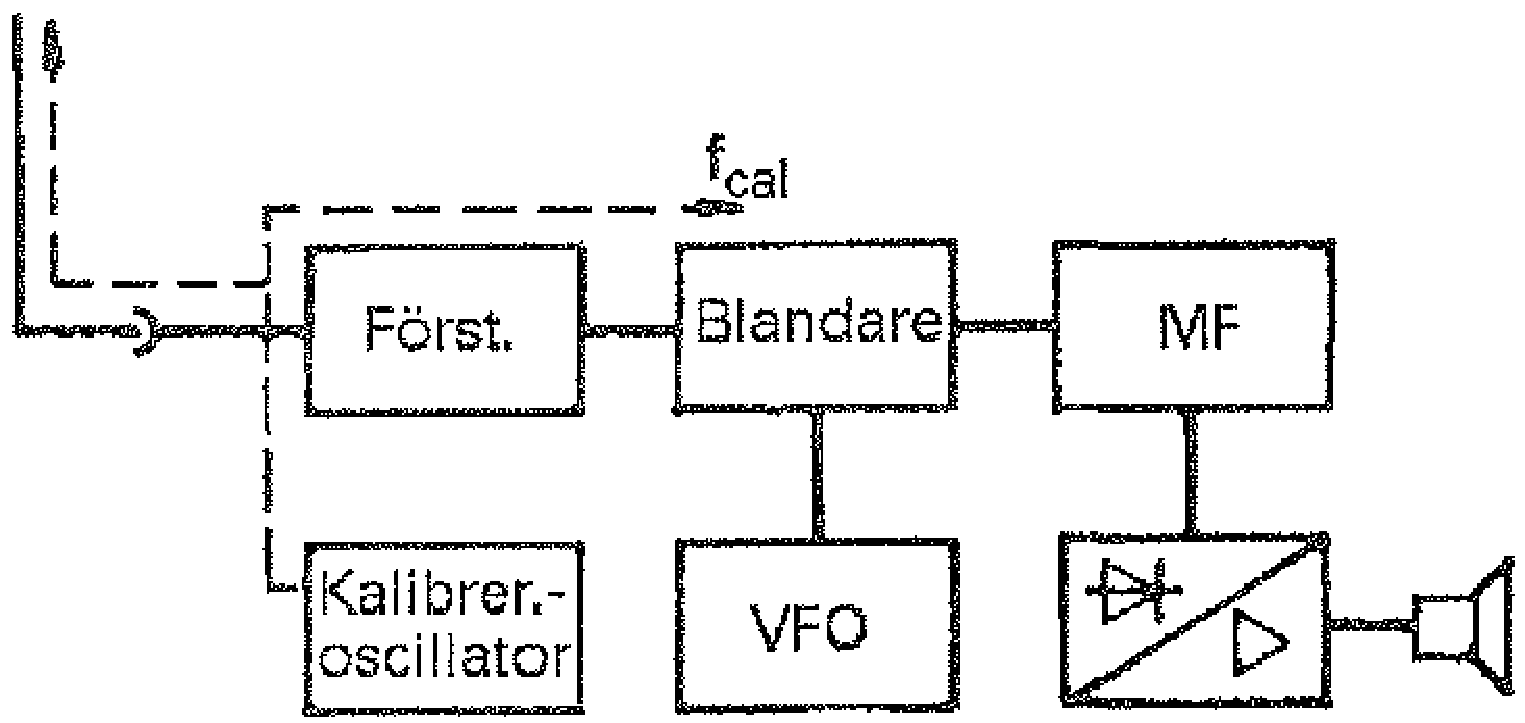
\includegraphics[width=0.5\textwidth]{images/cropped_pdfs/bild_2_8-07.pdf}
  \caption{Kalibreringsoscillator i mottagare}
  \label{fig:bildII8-7}
\end{wrapfigure}

En \emph{kalibreringsoscillator} (eng. \emph{calibration oscillator}) används
för att frekvenskalibrera andra apparaters inställningsskalor, som illustreras
i bild \ref{fig:bildII8-7}.
Den är kristallstyrd och avger särskilt precisa och frekvensstabila signaler.

Oscillatorsignalen förvrängs avsiktligt, så att det utöver grundfrekvensen även
skapas harmoniska övertoner.
En oscillator med till exempel grundfrekvensen 25~kHz avger på så sätt även
frekvenserna 50~kHz, 75~kHz, 100~kHz, 125~kHz osv.
Man får således en ''kalibreringsfrekvens'' för varje 25~kHz.

Detta övertonsspektrum kan sträcka flera 100~MHz upp.
Man ''nollsvävar'' apparat mot närmaste kalibreringsfrekvens och kan
kalibrera till exempel VFO-skalan.


gradering av nya skalor osv. för densamma.
Dagens mottagare och sändare har syntesoscillator och då behövs normalt ingen
kalibreringsoscillator.

\textbf{Not:}
Äldre trafikmottagare har VFO med LC-krets och ofta en inbyggd
kalibreringsoscillator.

En kalibreringsoscillator kan i sin tur behöva kalibreras.
Det enklaste sättet är då, att jämföra frekvensen på en känd rundradiosändare
på mellanvåg med kalibreringsoscillatorn.

\subsection{Brusmätbrygga}
\index{brusmätbrygga}
\index{Wheatstones brygga}

\begin{wrapfigure}{R}{0.5\textwidth}
  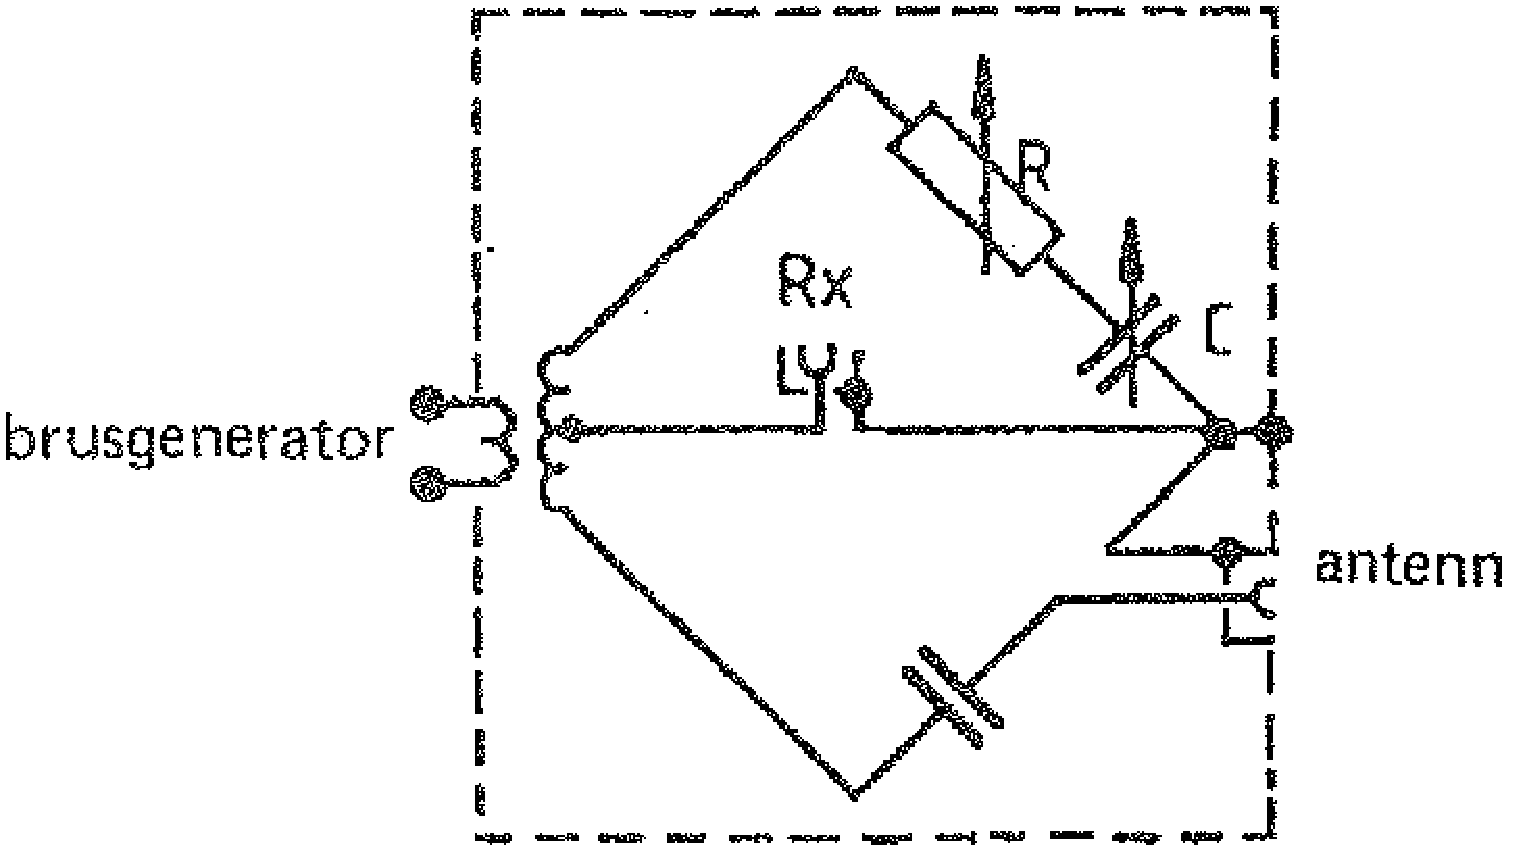
\includegraphics[width=0.5\textwidth]{images/cropped_pdfs/bild_2_8-08.pdf}
  \caption{Brusmätbrygga}
  \label{fig:bildII8-8}
\end{wrapfigure}

\emph{Brusmätbryggan} används vid mätning i antennsystem, så som illustreras i
bild \ref{fig:bildII8-8}.
Den består av en brusgenerator och en Wheatstonebrygga för mätning av
resistans och reaktans.

Till bryggan ansluts en antenn som mätobjekt och en mottagare som
nollindikeringsinstrument för brussignalen.
Mottagaren ställs in på den frekvens där mätvärden önskas.
Bruset hörs svagast när bryggan är injusterad.
Man kan då avläsas mätvärdena för \(R\) och \(X\).
Mäter man vid flera frekvenser, kan till exempel ett impedansdiagram upprättas.
Detta är med andra ord en äldre förlaga till en nätverksanalysator.

\subsection{Ståendevågmeter (SVF-meter)}
\textbf{
HAREC a.\ref{HAREC.a.8.2.1.3}\label{myHAREC.a.8.2.1.3}
}
\index{ståendevågmeter}
\index{SWR-meter}
\index{ståendevåg-förhållande (SVF)}
\index{Standing Wave Ratio}
\index{framåtgående effekt}
\index{forward power}
\index{bakåtgående effekt}
\index{backward power, reflected power}
\index{SVF}
\index{SWR|see {Standing Wave Ratio}}
\label{SVF}

\begin{figure}
  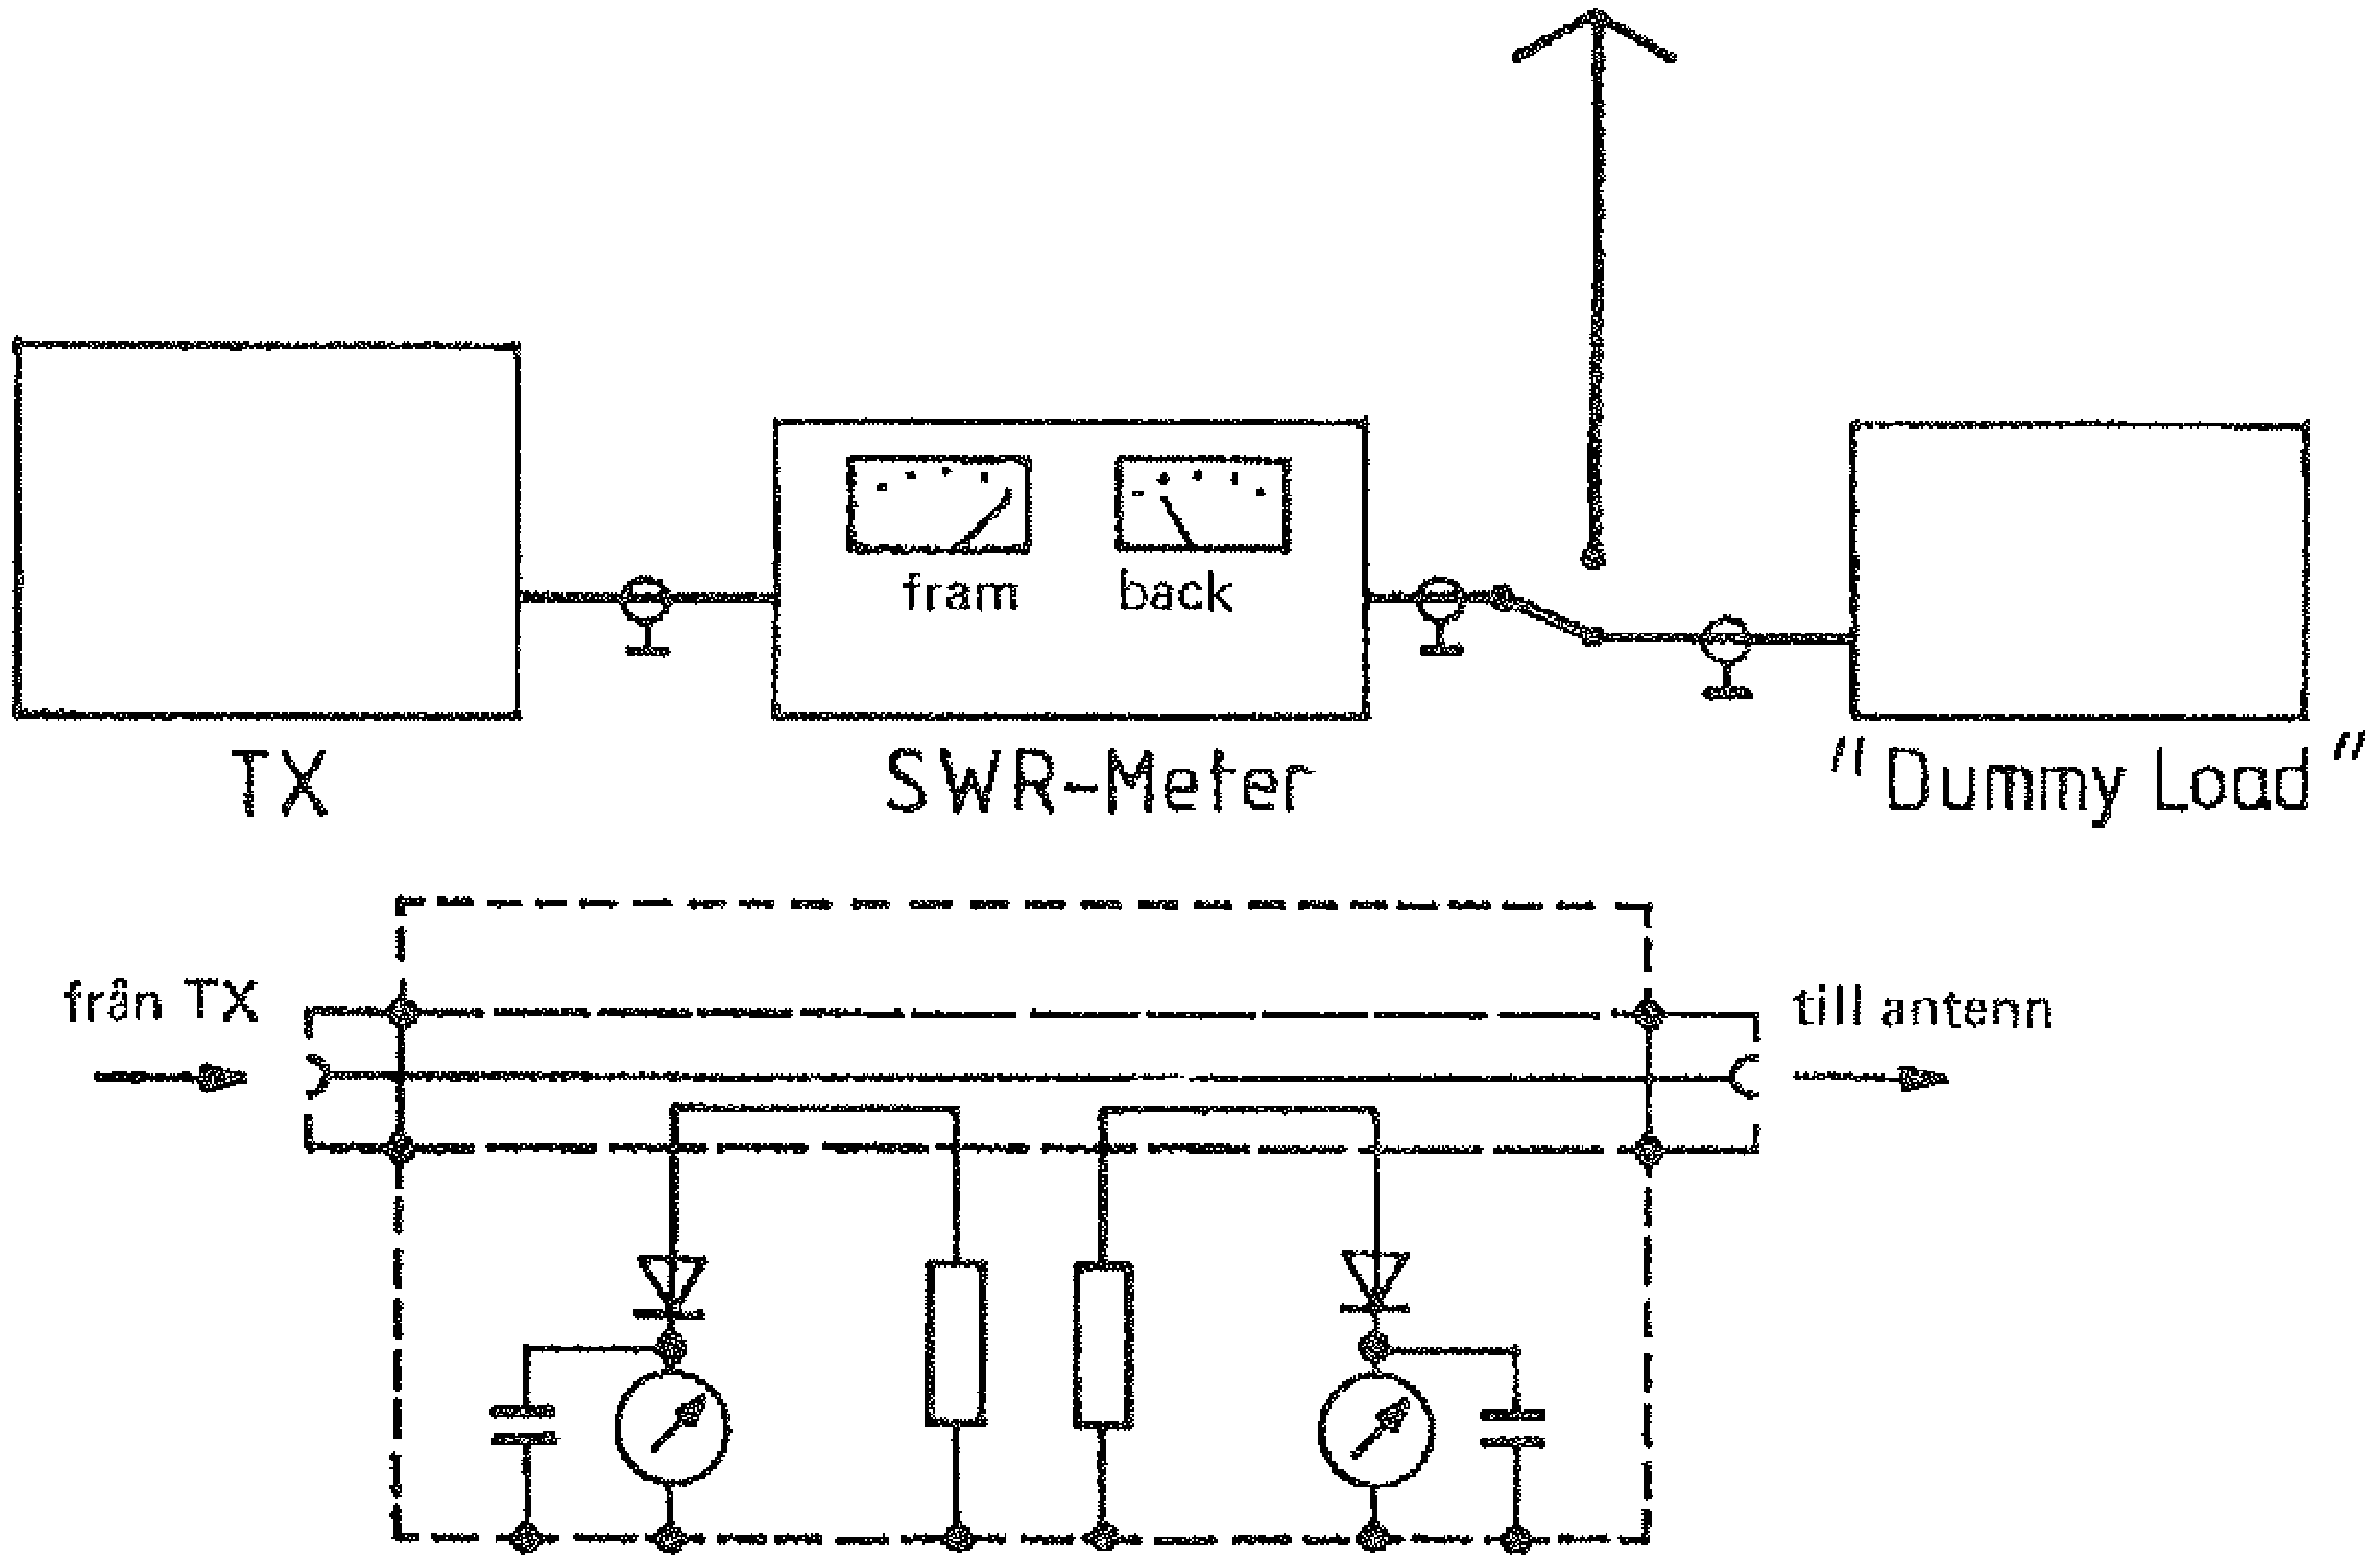
\includegraphics[width=\textwidth]{images/cropped_pdfs/bild_2_8-09.pdf}
  \caption{SVF-meter, princip och inkoppling}
  \label{fig:bildII8-9}
\end{figure}

När en transmissionsledning eller apparat ansluts till en annan med
avvikande impedans, kommer HF-energi att reflekteras i övergången.

Denna reflekterade energi kan mätas med en \emph{ståendevågmeter}
(eng. \emph{SWR-meter}) så som illustreras i bild \ref{fig:bildII8-9}.
Med \emph{ståendevåg-förhållande (SVF)} (eng. \emph{Standing Wave Ratio (SWR)}
menas förhållandet mellan den effekt som flyter framåt respektive bakåt i en
transmissionsledning.

Användningområden för SVF-meter är:
\begin{itemize}
\item Mätning av \emph{framåtgående effekt} (eng. \emph{forward power}).
\item Mätning av \emph{bakåtgående effekt} (eng. \emph{backward power, reflected power}).
\item Bestämning av \emph{SVF} (eng. \emph{SWR}).
\item Bestämning av resulterande, relativ effekt.
\end{itemize}

\textbf{Anmärkning:} Vid bestämning av absolut effekt måste
anslutningsimpedansen vara lika i instrument och transmissionsledning.

SVF-metern är ett av de mest användbara instrumenten vid HF-mätningar.
En SVF-meter kan ha separata instrument för fram- respektive backeffekt eller
ett gemensamt.

SVF-metern kan vara ständigt inkopplad till exempel mellan sändare och antenn, men
ska då kunna tåla effektutvecklingen.
En SVF-meter kan alstra övertoner, vilka kan medföra störningar.
Orsaken är olinjäriteten halvledardioderna i instrumentet.

\subsection{Frekvensräknare}
\textbf{
HAREC a.\ref{HAREC.a.8.2.1.5}\label{myHAREC.a.8.2.1.5}
}
\index{frekvensräknare}

\begin{wrapfigure}{R}{0.5\textwidth}
  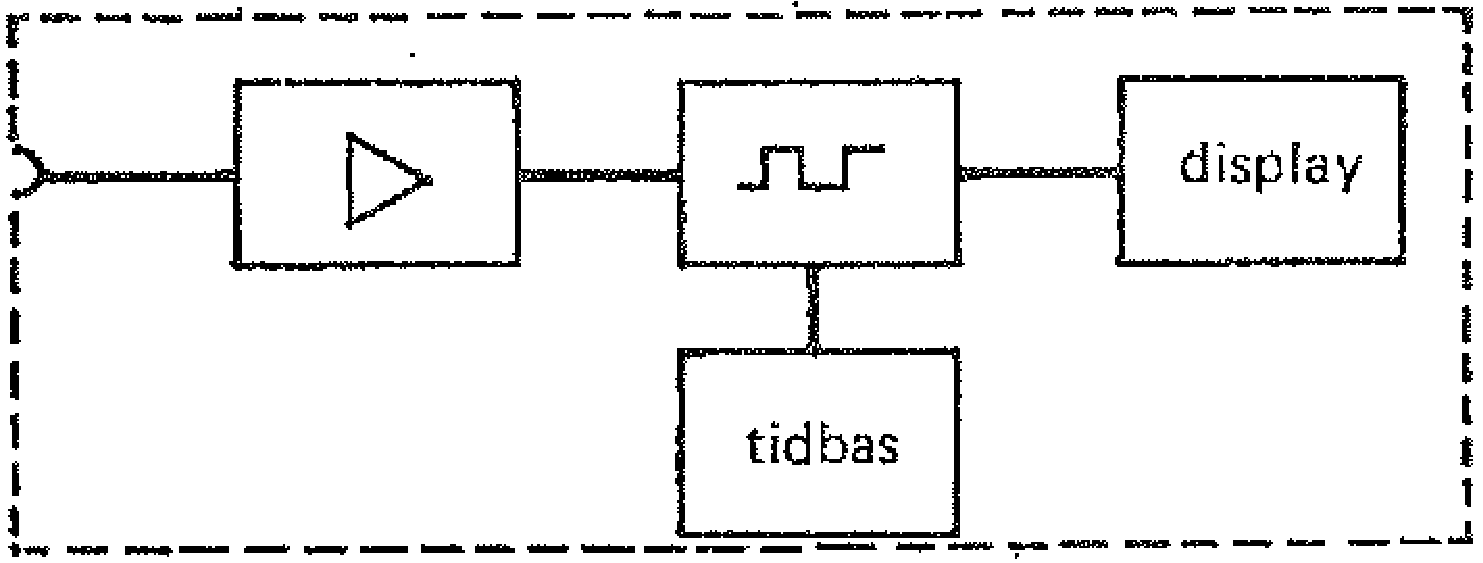
\includegraphics[width=0.5\textwidth]{images/cropped_pdfs/bild_2_8-10.pdf}
  \caption{Frekvensräknare}
  \label{fig:bildII8-10}
\end{wrapfigure}

\emph{Frekvensräknaren} (eng. \emph{frequency counter}), som är ett digitalt
instrument, används för att bestämma oscillatorfrekvensen i sändare,
mottagare m.m.

Bild \ref{fig:bildII8-10} illustrerar den schematiska bilden av en
frekvensräknare.
I frekvensräknaren räknas antalet svängningar \(E\) (från engelskans events)
i den aktuella inkommande signalen under en bestämd tidsenhet \(t\).
Först förstärks signalen i en analog förstärkare och omvandlas till
kantvågspulser i ingångsstegets triggerenhet.
När varje mätning börjar så kommer en räknare räkna hur många triggerpulser
som passerat fram tills dess den inställda tiden löpt ut.
Moderna räknare mäter även hur den första pulsen (eng. \emph{start event})
respektive sista pulsen (eng. \emph{stop event}) skiljer i tid, så att den
egentliga tiden kan användas, för att få en hög upplösning.
Frekvensen kan nu \emph{estimeras} med formeln

\(f_{est} = \dfrac{E}{t}\)

Gamla frekvensräknare hade en fix tid som den räknade över, och utan justering
av egentlig tid.
Dessa har en enkel princip och tiden valdes ofta för att få en enkel skalfaktor
mellan räknarens värde och frekvensen, genom att ha steg om 100~ms, 1~s, 10~s
osv.
Dessa räknare har dock problemet att för låga frekvenser så krävs lång
observationstid för att försäkra sig om en tillräckligt bra numerisk precision.
En variant av detta som framkom var den så kallade reciproka räknaren, som är
den nu förhärskande principen när man behöver precision, i den så mäts både
hur många event och tiden.
Detta gör att man kan låta tidbasen enkelt varieras med en pot eller extern
signal.

Ytterligare en förbättring som kom är att interpolera tiden för den inledande
och den avslutande pulsen gentemot tidbasens klocka, för att därför kunna
justera mätningen med ett bättre estimat på tiden det egentligen tog för de
räknade eventen att hända.
Med tidsupplösning på 1~ps-nivå kan därför 12~siffrors noggrannhet presenteras
för en mätning över 1~sekund, medan för gamla frekvensräknare med sin 10~MHz
oscillator gav 100~ns upplösning och därmed enbart 7~siffrors noggrannhet för
samma 1~sekund mätning.

De moderna frekvensräknarna har nu mer även filter som sammanställer flera
mätningar till en, och presenterar resultat överlappande.
Detta ger en uppfattad högre avläsningshastighet, men mätningarna är inte helt
oberoende.
Vissa frekvensräknare använder även linjärregression för att ytterligare
filtrera bort mätbrus.

Resultatet visas som siffror i ett fönster.
Noggrannheten i den s.k. tidbasen erhålls med en kristallstyrd oscillator
eller för dyrare instrument med en rubidiumnormal.
Man kan ofta ansluta en extern frekvensnormal med frekvens på 10~MHz,
vilket gör att man med moderna GPS-styrda oscillatorer kan få tillgång till
SI-definitionen av hertz till en nu mer modest kostnad även i ett hobbylabb.

\subsection{Dipmeter}
\index{dipmeter}

\begin{wrapfigure}{R}{0.5\textwidth}
  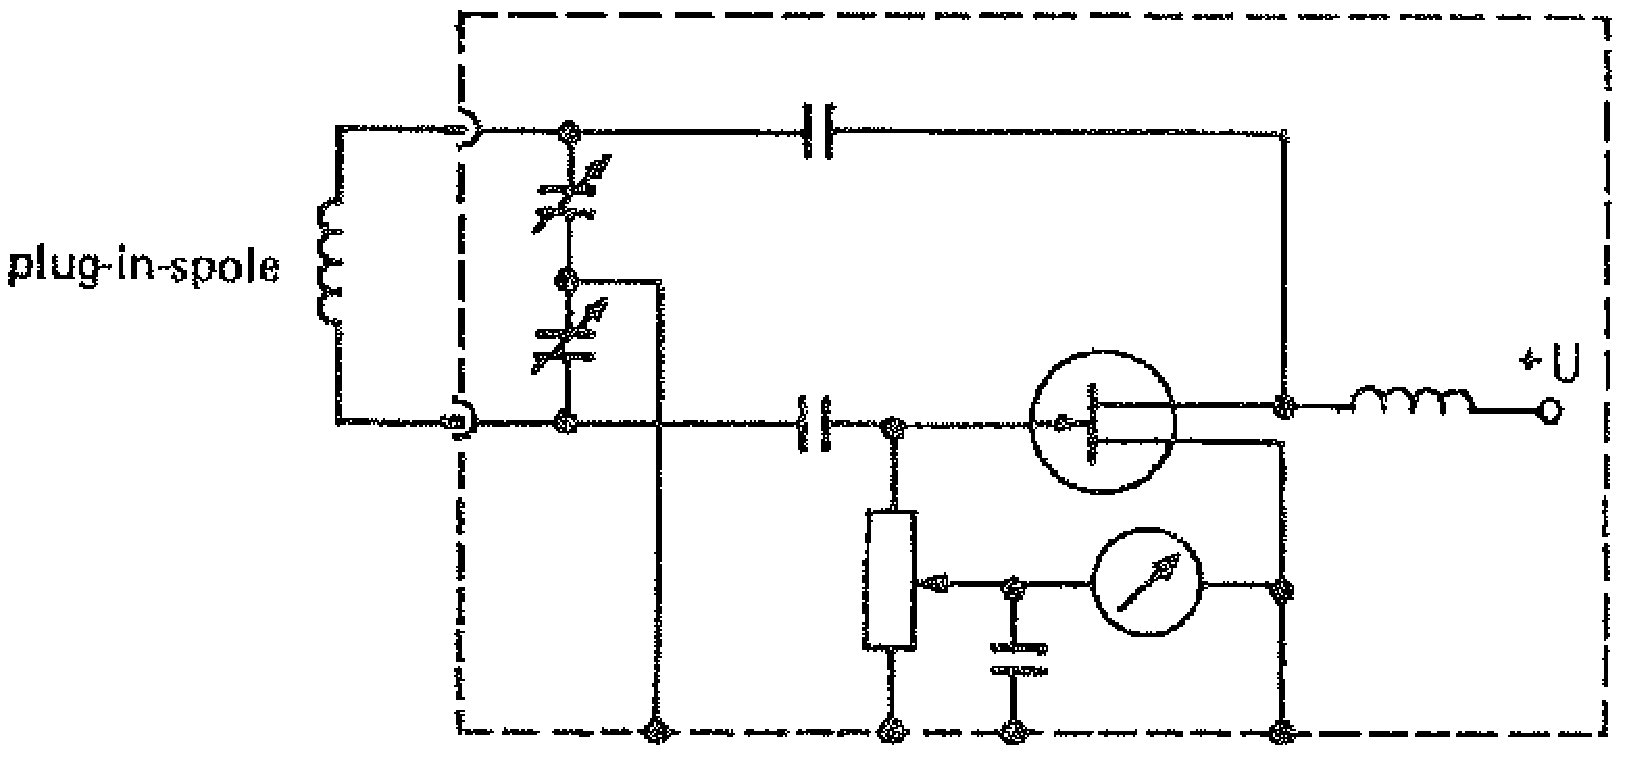
\includegraphics[width=0.5\textwidth]{images/cropped_pdfs/bild_2_8-12.pdf}
  \caption{Dip-meter}
  \label{fig:bildII8-12}
%\end{wrapfigure}

%\begin{wrapfigure}{R}{0.5\textwidth}
  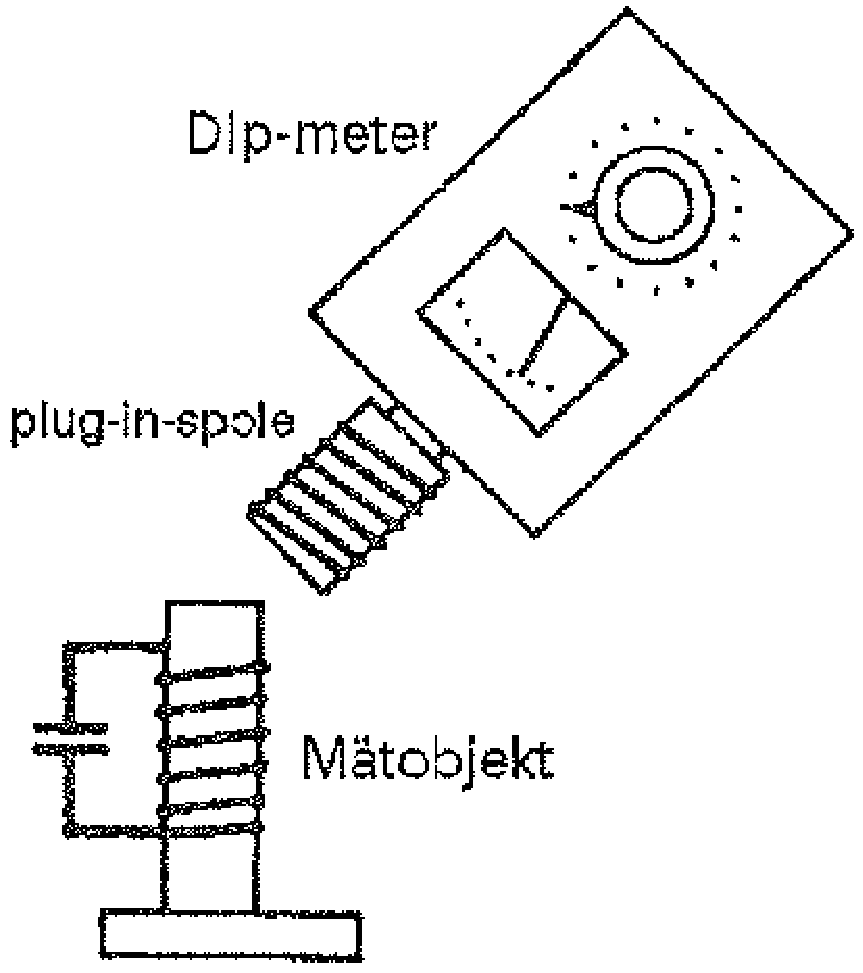
\includegraphics[width=0.5\textwidth]{images/cropped_pdfs/bild_2_8-13.pdf}
  \caption{Mätning med dip-meter}
  \label{fig:bildII8-13}
\end{wrapfigure}

\emph{Dipmetern} är i princip en oscillator med variabel frekvens och
utbytbara induktorer för olika frekvensområden, så som visas i bild
\ref{fig:bildII8-12}.
Den används för att bestämma resonansfrekvensen på passiva och aktiva
svängningskretsar samt vid bestämning av induktanser och kapacitanser.

Noggrannheten är ca 3~\%.

\textbf{Funktion:}
Instrumentet avger alternativt reagerar för en HF-signal med viss frekvens.
Resonansfrekvensen i dipmeterns svängningskrets är steglöst variabel och
frekvensvärdet kan avläsas på en skala.

Vid mätning av resonansfrekvensen i en passiv svängningskrets kopplas
dipmeterns induktor induktivt till kretsen så som visas i bild
\ref{fig:bildII8-13}.
När resonansfrekvensen i kretsen och dipmetern överensstämmer, ändras
belastningen i dipmeterns svängningskrets varvid instrumentet uppvisar en
strömminskning -- en ''dip''.
Frekvensen avläses då på skalskivan.

Vid mätning på en aktiv svängningskrets, dvs. som drivs av någon HF-källa,
uppstår i stället en strömökning vid resonans vilket också visas på
instrumentet.

Induktansen i en svängningskrets kan bestämmas med dip-metern, om kapacitansen
är bekant.
På motsvarande sätt kan en obekant kapacitans bestämmas om induktansen i
svängningskretsen är bekant.

Namnet griddipmeter kommer från elektronrörsepoken.
Ändringar i gallerströmmen (grid current) i ett oscillatorkopplat elektronrör
används som indikation på att en svängningskrets är i resonans.
Då minskar gallerströmmen -- det blir en ''ström-dip''.
Numera används en transistor i stället för röret och instrumentet benämns
dip-meter.

\subsection{Oscilloskop}
\textbf{
HAREC a.\ref{HAREC.a.8.2.1.6}\label{myHAREC.a.8.2.1.6}
}
\index{oscilloskop}

\begin{figure}
  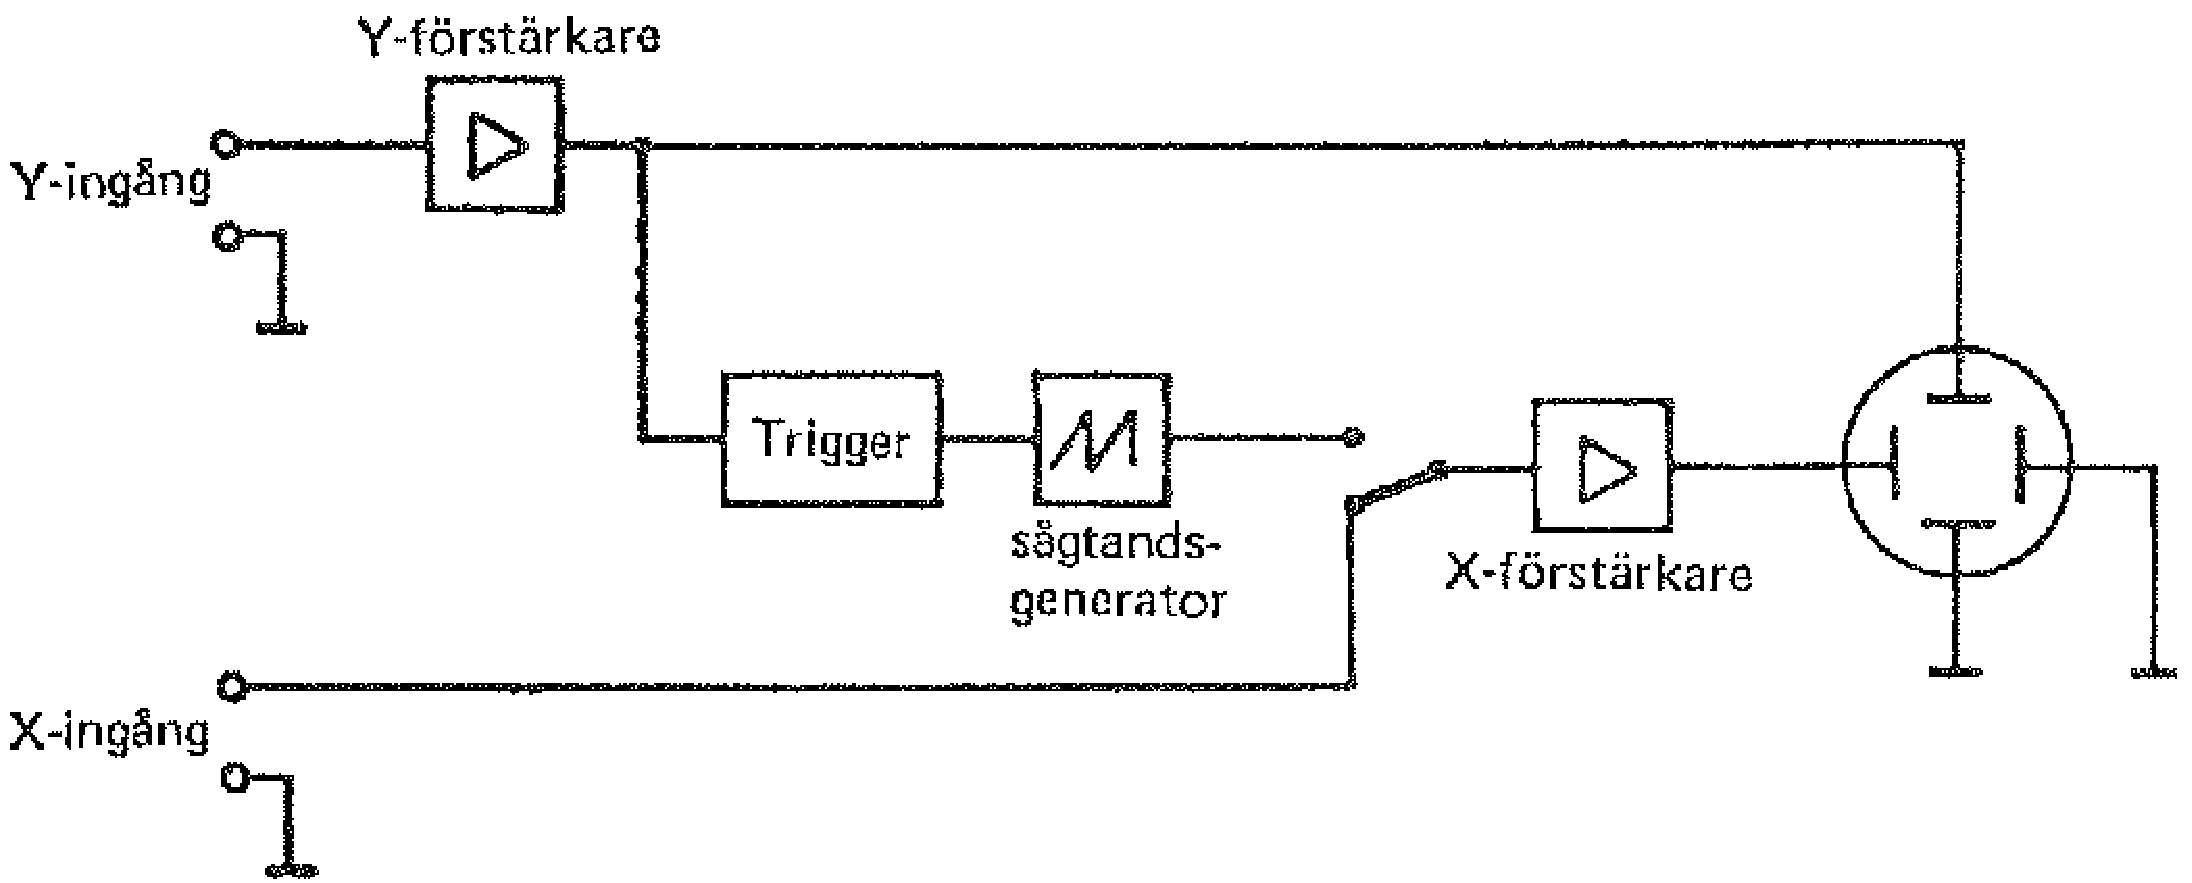
\includegraphics[width=\textwidth]{images/cropped_pdfs/bild_2_8-14.pdf}
  \caption{Oscilloskop}
  \label{fig:bildII8-14}
\end{figure}

\emph{Oscilloskopet} (eng. \emph{oscilloscope}) är ett mycket användbart
instrument.
Mycket snabba förlopp kan med fördel studeras på en oscilloskopskärm.

Spänningsförlopp kan visas som funktion av tiden.
Tillsammans med andra instrument kan frekvenskaraktäristiken i filter,
modulationskvalitet osv. åskådliggöras.

Oscilloskopet består av ett katodstrålerör, där styrningen av katodstrålen sker
med hjälp av X- och Y-förstärkare och en s.k. triggerförstärkare.
Den signal som ska mätas ansluts vanligen till Y-förstärkaren medan en
tidbasgenerator som alstrar en sågtandsformad signal ansluts till X-förstärkaren.
Bild \ref{fig:bildII8-14} visar ett blockschema på oscilloskop.

Moderna oscilloskop digitaliserar signalen efter ingångsförstärkaren,
och läggs sedan i minne, där den sågtandsformade signalen är ersatt med en
räknare som placerar det i minnet.
Sen presenteras bilden på bildskärmen eller på en ansluten dator.

Gemensamt för analoga och digitala oscilloskop är i stort samma handhavande.

Man ansluter en eller flera signaler till ingångarna, justerar ingångssteget
så att hela vågformen fångas och att det är god amplitud, så den syns men inte
klipps.
Ibland väljer man att göra vågformerna mindre, för att man ska kunna
arrangera dem på ett bra sätt på skärmen.
Ibland väljer man att klippa vågen för att man enbart vill se tiden för en
kant tydligt.

En viktig sak för att få en tydlig bild på bildskärmen är att triggpunkten,
den punkt där mätningen av signalen börjar, är vald så att man inte får dubbla
eller otydliga bilder.
Valet av triggpunkt sker ofta automatiskt men om signalen som ska mätas är
väldigt flack eller har många nollgenomgångar kan triggpunkten bli felaktig.
För att lösa problemet med suddiga eller dubbla bilder så brukar man manuellt
justera triggpunkten så att man får en tydlig bild.

Man justerar också tidbasen för att ha rätt skala på tidsaxeln, så man ser en
eller ett fåtal cykler, eller ibland över längre tid för att se variationer.
Man kan också fördröja svepet för att kunna se en viss del efter triggpunkten.

Oscilloskop har nu mera ofta inbyggda funktioner för mätning.
Det är behändigt att snabbt få en uppfattning om periodtider, frekvenser,
amplituder m.m. men dessvärre blir mätprecisionen ofta kraftigt lidande, och
det ska inte övertolkas.
Till exempel är frekvensmätningen inte bättre än hur bra placeringen av markörerna är,
så det är sällan tillförlitligheten är bättre än 2 siffrors noggrannhet.

Rätt använt är oscilloskop dock ett fantastiskt mätinstrument.

\subsection{Spektrumanalysator}
\textbf{
HAREC a.\ref{HAREC.a.8.2.1.7}\label{myHAREC.a.8.2.1.7}
}
\label{spektrumanalysator}

En \emph{spektrum-analysator} (eng. \emph{spectrum analyzer}) visar amplituden
för olika frekvenser över ett visst frekvensområde.
Detta är som kontrast till oscilloskopet som visar amplitud för en signal
över tiden.

Spektrumanalysatorn kan liknas vid en mottagare, men med en viktig skillnad:
där en mottagare har ett eller flera avstämda ingångssteg, som ska förhindra
mottagaren att påverkas av signaler som ligger mer eller mindre nära den
önskade signalen, har spektrumanalysatorn en vidöppen ingång.

Spektrumanalysatorn är ett mätinstrument, och ska kunna presentera de
signaler som matas in på dess ingång, utan att signalerna ska påverkas på
något sätt.

Detta ställer höga krav på spektrumanalysatorns konstruktion.
Den måste kunna tåla starka signaler, utan att en mätning på en svag signal i
närheten påverkas.

Spektrumanalysatorerna finns också i två olika typer.
Den ena arbetar med svepteknik, och sveper över ett viss del av
frekvensspektrumet.
Den andra typen kallas för \emph{realtidsanalysator}, och är kapabel att för
ett givet ögonblick spela in ett spektrum digitalt för senare analys av
innehållet.

Det vi fortsättningsvis beskriver i detta kapitel, är den svepande
spektrumanalysatorn, vilket också är den vanligaste typen för
service tillämpningar.

En spektrum-analysator består förenklat av en svep-bar oscillator,
variabelt filter på mellanfrekvensen, en detektor och ett ställbart
filter från detektorn.

Den variabla oscillatorn sveper så att det tänkta frekvensområdet täcks,
ofta med ett bestämt antal punkter, till exempel 801, där varje punkt är mätning på
en specifik frekvens.
Ibland kan man anpassa antalet punkter för att få mätningen gå snabbare,
mot att man får en lägre upplösning.

Filtret sätter bandbredden på mätningen, och det kan gå i 1--3 steg, till exempel
3~Hz, 10~Hz, 30~Hz, osv. till 3~MHz.
För vissa specifika mätändamål, som till exempel för EMC mätningar, behöver man ha
filter av rätt bandbredd och dessa är extra optioner.

Filtret, vars inställning brukar kallas för \emph{Resolution Bandwidth},
fungerar som ett fönster, där fönstret släpper in de signaler som finns i det
spektrum som man önskar studera. 

Om analysatorn inte skulle ha något filter skulle den ta in alla signaler som
finns inom dess specificerade frekvensområde.

Ett brett filter släpper igenom ett större frekvensområde och är användbart för
signaler med större bandbredd.
Ett smalare filter är att föredra för signaler med smalare bandbredd.

Ett brett filter innebär också att analysatorn kan svepa snabbare.
Det är då lättare att kunna detektera signaler som är kortvariga.
Ett smalare filter innebär att analysatorn måste svepa långsammare, men kan då
istället hitta signaler som inte skulle ha synts med det bredare filtret.

Detta filter har också en annan egenskap som är viktig -- ett brett filter
släpper också igenom mer brus, vilket påverkar den lägsta brusnivån som
analysatorn kan presentera.

För att nå högre känslighet kan man välja smalare filter.
Ju smalare filter, desto högre känslighet, men också ett långsammare svep över
det aktuella frekvensområdet.

\subsubsection{Fördjupning}

På en spektrumanalysator ställs stora krav på känslighet och förmåga att hantera
starka signaler i närheten av en svag men önskad signal utan att falska signaler
påverkar instrumentet.
Kraven har medfört att kostnaden för instrumentets uppbyggnad och ingående
komponenter under lång tid har varit mycket hög.

Under många decennier har sändaramatörer därför varit hänvisade till
marknaden för begagnade instrument som haft minst tio till tjugo år på nacken.

Det är bara för några år sedan som det har kommit produkter på marknaden som nu
kommit ner i kostnadsnivåer som inneburit att radioamatörer kan köpa dessa
instrument, i nyskick.

En modern spektrumanalysator av dyrare snitt erbjuder också en möjlighet att
analysera den modulerade signalen.
Sålunda förekommer instrument på marknaden som är specialdesignade att
analysera signaleringsinnehållet i olika system, till exempel Bluetooth, olika
Wi-Fi- och mobilsystem.

För en specifik mätning över ett visst frekvensspektrum, kan man ställa in en
s.k. start-frekvens, samt motsvarande stopp-frekvens för spektrumet ifråga.
Analysatorn kommer då att svepa, från startfrekvensen, till stoppfrekvensen.
Man kan också att välja en frekvens mitt i spektrumet, och därefter ett
valfritt s.k. span.
\emph{Span} betecknar det frekvens-spann som är önskvärd för att man ska
kunna studera signalerna inom det aktuella spektrumet.

För att kunna göra bättre avläsningar kan man sätta markörer, så att man kan
avläsa frekvens och amplitud för den punkten.
Ibland sätter man dubbla frekvensen för att avläsa skillnaden i amplitud,
vilket kan vara relevant för filter eller avläsa den relativa styrkan på ett
sidband.

Detektorn kan vara topp-detektor eller RMS detektor, det kan finnas flera.
För specifika mätändamål som till exempel EMC mätningar behöver man specifik detektor.
Det är viktigt att välja rätt detektor när signalen ska presenteras.
Valet av detektor kan påverka den presenterade nivån med flera dB.

Det finns olika detektorer beroende på hur man vill ha signalen presenterad.
Det finn toppvärdesindikerande (Auto-peak, max peak, min peak) detektorer som
indikerar signalens toppvärden.
Det finns medelvärdesbildande (\emph{Average}, \emph{Sample}) detektorer som, om
instrumentet arbetar med digitalteknik, plockar ögonblickliga mätvärden
slumpmässigt.
Det finns också speciella detektorer ( s.k. Quasi-Peak) som används för att
mäta enligt specifika EMC-mätningar.

En viktig detektor att komma ihåg är den s.k. RMS-detektorn.
Den utvecklades för att kunna mäta på digitalt modulerade signaler, ofta med
varierande fas- och amplitudinformation.

Denna detektor är att rekommendera för att mäta på digitalt modulerade signaler.
Den finns oftast i lite modernare analysatorer.

En vanlig Average- eller Sample-detektor enligt ovan, förväntar sig att
RF-signalens förlopp är  i stort sett återkommande konstant, vilket är fallet
med analoga signaler som består av en bärvåg.

En digitalt modulerad signal har ett innehåll som förändras hela tiden, oftast
både till fas och amplitud.

RMS-detektorn läser in -- samplar -- den digitalt modulerade signalen och tar
konstant mätvärden ur den fasvarierande RF-signalen.
Den följer RF-signalens förändrade innehåll.

Denna detektor är därför utmärkt att använda för att mäta på digitalt
modulerade signaler. till exempel Bluetooth eller Wifi-signaler, men även de digitala
system vi har inom amatörradion, då dessa signaler innehåller förändringar i
fas- och amplitud.

Den kan självklart också användas för att mäta på analoga signaler.
Att den plockar ögonblicksmätvärden även på en analog signal gör alltså inget.

Efter detektorn finns ett filter, ofta benämnt med videobandbredd, som
medelvärdesbildar detektorns amplitud estimat över tiden.
Oftast regleras det automatiskt med bandbredden på filtret, eftersom smalare
filter behöver proportionerligt längre tid för att ge ett bra resultat.
Sveptiden beror därför på antalet punkter för frekvenser, bandbredd på filtret
och videobandbredden.
Ibland kan man styra videobandbredden manuellt för att få en längre tid, då
det kan vara gynnsamt för att få en tydligare bild, dvs. ta bort brus och
störningar som enbart skapar variationer för att man inte observerar ett bra
medelvärde.
Videobandbredden påverkar alltså inte själva mätresultatet, utan är enbart till
för att användaren lättare ska kunna avläsa mätningen.

\subsection{Signalgeneratorn}
\textbf{
HAREC a.\ref{HAREC.a.8.2.1.4}\label{myHAREC.a.8.2.1.4}
}

\emph{Signalgeneratorn} (eng. \emph{signal generator}) är ett instrument, som
namnet antyder, genererar en signal, i detta fall en radiofrekvent signal.

Detta instrument kan användas för att till exempel testa mottagare, eller för att att
generera en eller flera kontrollerade signaler för att till exempel testa
förstärkarsteg.

Äldre signalgeneratorer var oftast uppbyggda runt en svängningskrets, och drev
ofta i frekvens när de värmdes upp.
De var sålunda inte stabila.
Senare generatorer arbetade med frekvenssyntes, och var att föredra i detta
sammanhang.

Den kan också användas för att generera en testsignal, som man matar in på en
mottagares ingång, för att sedan kunna följa signalen med en spektrumanalysator
(se \ref{spektrumanalysator}).

En bra signalgenerator ska ha förmågan att ge en så ren signal som möjligt,
där övertoner och sidband av olika slag är så låga som möjligt.
Ofta genererar generatorn ett egenbrus runt den inställda signalen.
Detta brus avtar, ju längre bort man kommer från den inställda signalen.
Detta brus ska förstås vara så lågt som möjligt.

En annan önskvärd parameter är möjligheten at kunna reglera den radiofrekventa
utnivån över ett stort område.
Signalgeneratorer innehåller oftast någon form av mätfunktion för att kunna
mäta nivån.

En fördel är om signalgeneratorn har en möjlighet att själv skapa modulation,
till exempel AM- eller FM-signaler.
Det kan emellanåt finna en inbyggd lågfrekvensgenerator, där man kan ställa in
önskad frekvens fär att till exempel generera en ton.
I detta sammanhang brukar det också finnas möjlighet att justera
modulationsgraden för AM, eller deviationen för FM-signalen.

\subsection{Nätverksanalysator}
\label{nätverksanalysator}
\label{network analyzer}
\label{antennanalysator}
\label{skalär nätverksanalysator}
\label{Scalar Network Analyzer (SNA)}
\label{SNA}
\label{tracking generator}
\label{vektornätverksanalysator}
\label{Vector Network Analyzer (VNA)}
\label{VNA}

En \emph{nätverksanalysator} (eng. \emph{network analyser}) används för att
mäta hur mycket signal som går igenom en koppling, till exempel filter eller
förstärkare, eller hur mycket signal som reflekteras tillbaka från till exempel en
antenn.
Ibland kallas detta även för \emph{antennanalysator} i amatörradiosammanhang.

En nätverksanalysator som enbart kan mäta amplituder kallas ibland för
\emph{skalär nätverksanalysator} (eng. \emph{Scalar Network Analyzer (SNA)}).
En spektrumanalysator med en så kallad \emph{tracking generator}, som genererar
en signal med samma frekvens som man analyserar, kan agera SNA.
En signalgenerator med svepfunktion kan också agera SNA.

En nätverksanalysator som mäter fasen både på utgående och inkommande signal
kan även mäta fasförskjutningen, och då kan man representera fasen både som
komplex storhet eller med polära koordinater, dvs. amplitud och fas.
En sådan nätverksanalysator kallas för \emph{vektornätverksanalysator} (eng.
\emph{Vector Network Analyzer (VNA)}).

Användningsmässigt liknar en nätverksanalysator en spektrum-analysator, men
med flera väsentliga skillnader.
För att få korrekt mätning av amplitud och fas läggs större vikt vid att göra
\emph{kalibrering} (eng. \emph{calibration}), något som görs för att kompensera
varierande amplitud och fas för olika frekvenser.
Vid kalibrering använder man ofta \emph{last} (eng. \emph{load}),
\emph{kortslutning} (eng. \emph{short}) samt \emph{öppen port} (eng.
\emph{open}) mätning av kalibreringsreferenser.
För två-ports mätning använder man även en \emph{överföring} (eng.
\emph{through}) för att få port-till-port egenskaperna korrekt.
Efter kalibrering av instrumentet så korrigeras mätningarna, och ibland kan
skillnaderna vara drastiska.

Nätverksanalysatorn har därtill ofta ett stort antal olika sätt att presentera
mätresultaten så att man kan mäta enligt \emph{scatter-modellen},
\emph{return loss (RL)}, \emph{VSWR}, \emph{Smith-diagram} och så vidare.
Det gör att en nätverksanalysator kan vara ett kraftfullt verktyg som korrekt
använt kan ge god insikt i hur en krets beter sig.
